\subsection{NVFP4 Pretraining}\label{sec:nvfp4}
\begin{table*}[!hbt]\small\centering
\renewcommand{\arraystretch}{1.3}
\setlength{\tabcolsep}{10pt}
\caption{Precision by Layer Type}
\label{table:precision_by_layer}
\begin{tabular}{l|c|p{6cm}}
\toprule
\textbf{Layer Type} & \textbf{Format} & \textbf{Rationale}\\
\midrule
All Linear Layers Unless Otherwise Noted & NVFP4 &\\
\midrule
Final 15\% of Network & BF16 & Promote training stability at scale\\
\midrule
Latent Projections & BF16 & Strategically kept in BF16 as step-time impact is negligible\\ 
\midrule
MTP Layers & BF16 & Preserves multi-token prediction capabilities \\
\midrule
QKV \& Attention Projections & BF16 & Maintain fidelity of few attention layers\\
\midrule
Mamba Output Projection & MXFP8 & Mitigates high incidence of underflows observed when quantizing this layer to NVFP4 at smaller scales \\
\midrule
Embedding Layers & BF16 &\\ 
\bottomrule
\end{tabular}
\end{table*}


Nemotron 3 Super was trained with the NVFP4 pretraining recipe detailed in the Nemotron 3 white paper \citep{nvidia2025nvidianemotron3efficient}. All linear layers, unless otherwise noted in Table \ref{table:precision_by_layer}, are trained using the open-source NVFP4 GEMM kernels provided by Transformer Engine with the cuBLAS backend \citep{NVIDIA_TransformerEngine_PR2177} for fprop, dgrad, and wgrad GEMMs. This framework performs quantization of weights, activations, and gradients to NVFP4 according to the scheme first introduced in \citet{nvidia2025pretraininglargelanguagemodels}. Weights are quantized to NVFP4 using two-dimensional (2D) block scaling to maintain consistency between quantized weights in the forward and backward pass. Gradients and activations are quantized to NVFP4 using one-dimensional (1D) blocks along the GEMM reduction axis. Random Hadamard Transforms (RHTs) are performed on inputs to wgrad and stochastic rounding is applied to gradient tensors. The NVFP4 format utilizes an E2M1 element format with 16-element micro-blocks, E4M3 micro-block scaling factors, and a second-level FP32 global scale. Nemotron 3 Super showcases large-scale stable training in NVFP4 up to 25T tokens.


During the training of Nemotron 3 Super, we observed a growth in the number of zero-valued weight gradient elements and investigated the root cause to validate training health. Magnitude patterns emerged within some expert layers, characterized by the norms of FC1 output channels and corresponding FC2 input channels converging toward zero (Figure \ref{fig:nvfp4_magnitude_patterns_super}). By the end of pretraining, zero-valued weight gradient elements accounted for 7\% of total parameters, appearing to correlate with the magnitude patterns. We believe that NVFP4 quantization increases the incidence of true zeros in the weight gradients that could have been more easily be represented by BF16 or MXFP8. Low-norm channels likely attenuate quicker when these layers are trained in NVFP4.

\begin{figure}[h]
    \centering
    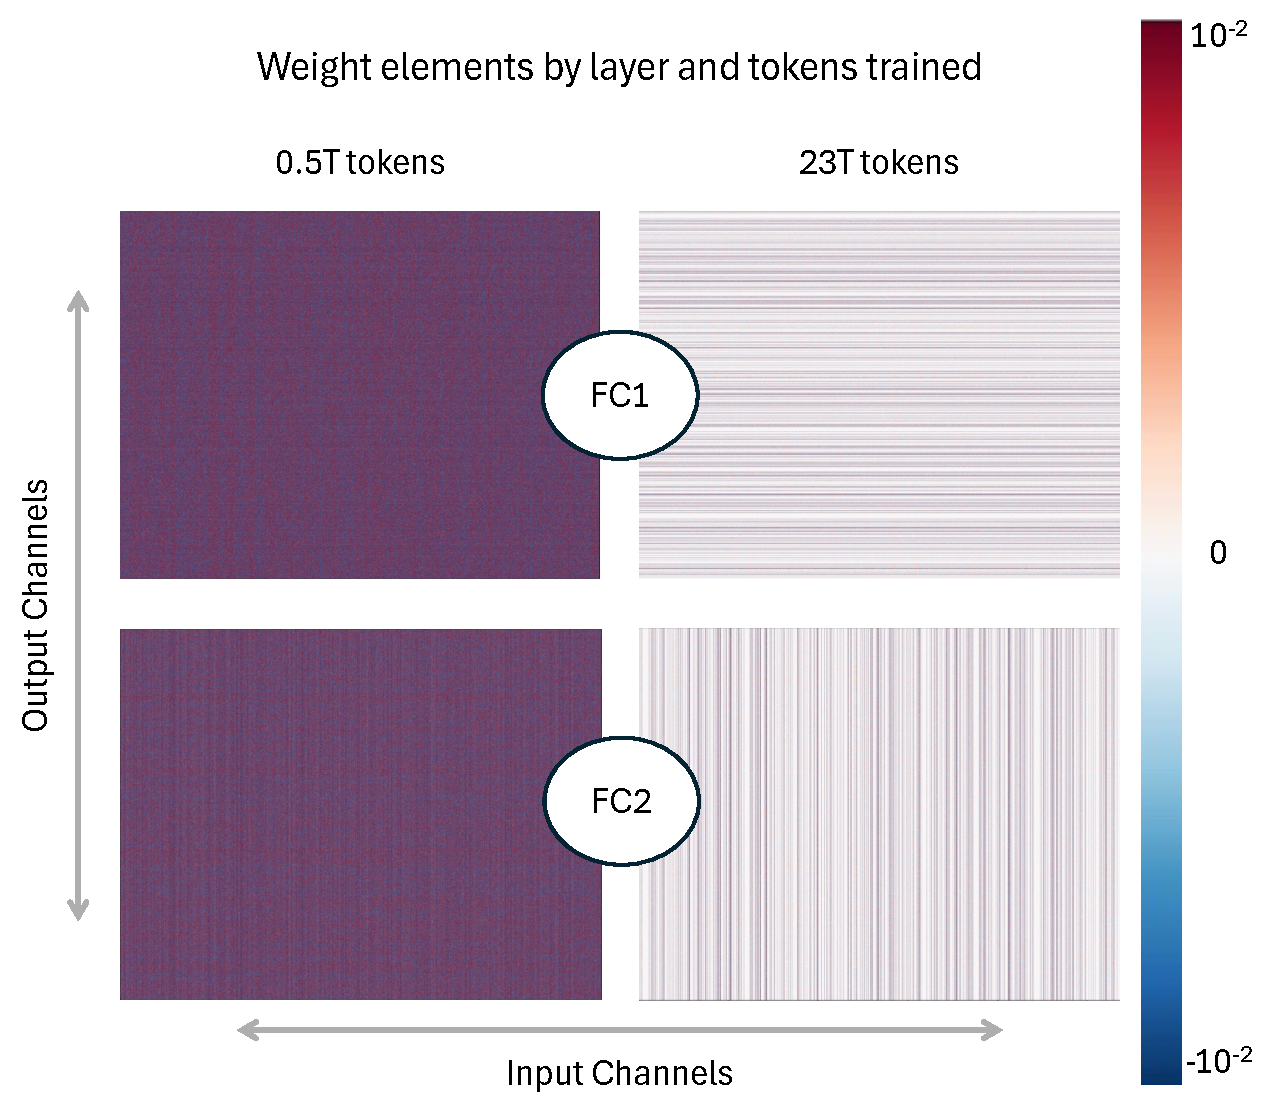
\includegraphics[width=0.55\textwidth]{figures/nvfp4_magnitude_patterns_super.pdf}
    \caption{Channel Magnitude Patterns in Weights of Expert Layers in Nemotron 3 Super. Patterns emerge as training progresses. Top: Early layer routed expert FC1 weight matrix at 0.5T tok and 23T tok. Bottom: Early layer routed expert FC2 weight matrix at 500B tok and 23T tok. Low-norm output channels of FC1 align with low-norm input channels of FC2.}
    \label{fig:nvfp4_magnitude_patterns_super}
\end{figure}

\begin{figure}[h!]
    \centering
    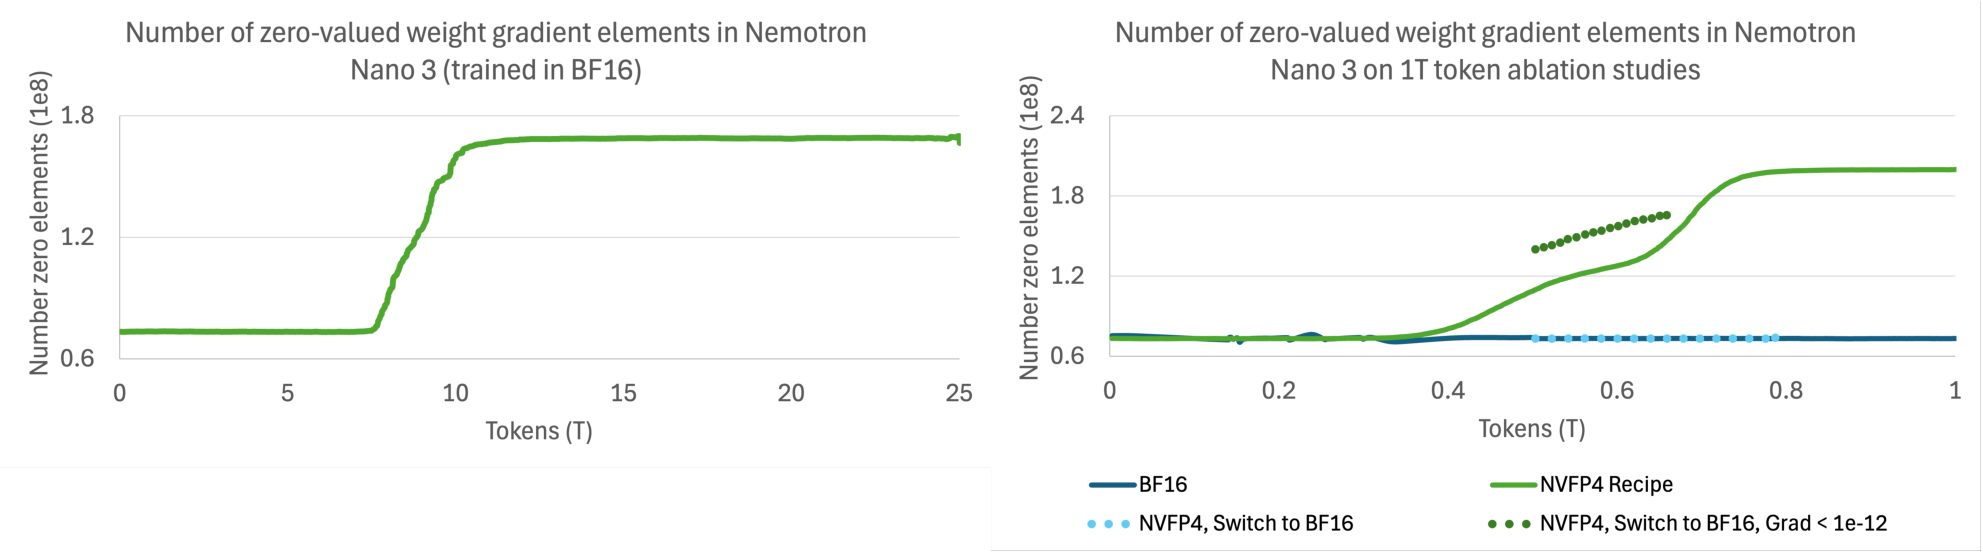
\includegraphics[width=1\textwidth]{figures/nvfp4_num_zeros_in_nano_during_training.pdf}
    \caption{Number of Zero-Valued Weight Gradient Elements on Nemotron 3 Nano.
Left: Released Nemotron Nano 3 model \citep{nvidia2025nemotron3nanoopen} trained to 25T tokens in BF16. Right: Ablation study trained to 1T tokens in BF16 and with our NVFP4 recipe. The NVFP4 model at 1T tokens reaches a similar zero-valued weight gradient count as the BF16 model at 25T tokens. Switching from NVFP4 to BF16 at 0.5T tokens causes zero-valued weight gradients to return to baseline levels. The high prevalence of small-magnitude gradients (<1e-12) in BF16 suggests NVFP4 quantization underflows already-small values to zero.}
    \label{fig:nvfp4_num_zeros_in_training_nano}
\end{figure}

We compare identical Nemotron 3 Nano models \citep{nvidia2025nemotron3nanoopen} trained for 1T tokens in BF16 and in NVFP4 and find that NVFP4 pretraining produces roughly 3x more zero-valued weight gradients at the same token horizon. When a partially trained NVFP4 model is switched back to BF16, the number of zero-valued weight gradients returns to baseline levels. The BF16 model still contains many small-magnitude gradients (<1e-12), but NVFP4 quantization underflows these values to zero (Figure \ref{fig:nvfp4_num_zeros_in_training_nano}). We sampled weight, activation, and gradient tensors from routed expert layers and observed high rates of underflow in dgrad of FC2 at 500B tokens, primarily because two-dimensional weight quantization blocks span high and low magnitude channels. Underflows in dgrad of FC2 create zeros in wgrad of FC1 through backpropagation of the gradient. At 750B tokens, we observe high rates of underflow in fprop of FC1, creating zeros in wgrad of FC2 (Figure \ref{fig:nvfp4_wgrad_zeros}). The 1T-token NVFP4 model behaves similarly to a much longer-trained BF16 model. After 10T tokens, the released Nemotron 3 Nano model, trained in BF16, \citet{nvidia2025nemotron3nanoopen} reaches a similar number of zero-valued weight gradient elements as the NVFP4 model trained to 1T tokens (Figure \ref{fig:nvfp4_num_zeros_in_training_nano}) and inspection of weight matrices in early expert layers revealed a similar channel magnitude pattern. These conclusions on the Nemotron 3 Nano architecture give insights into the channel magnitude patterns and growth in zero-valued weight gradient elements in Nemotron 3 Super.


\begin{figure}[h!]
    \centering
    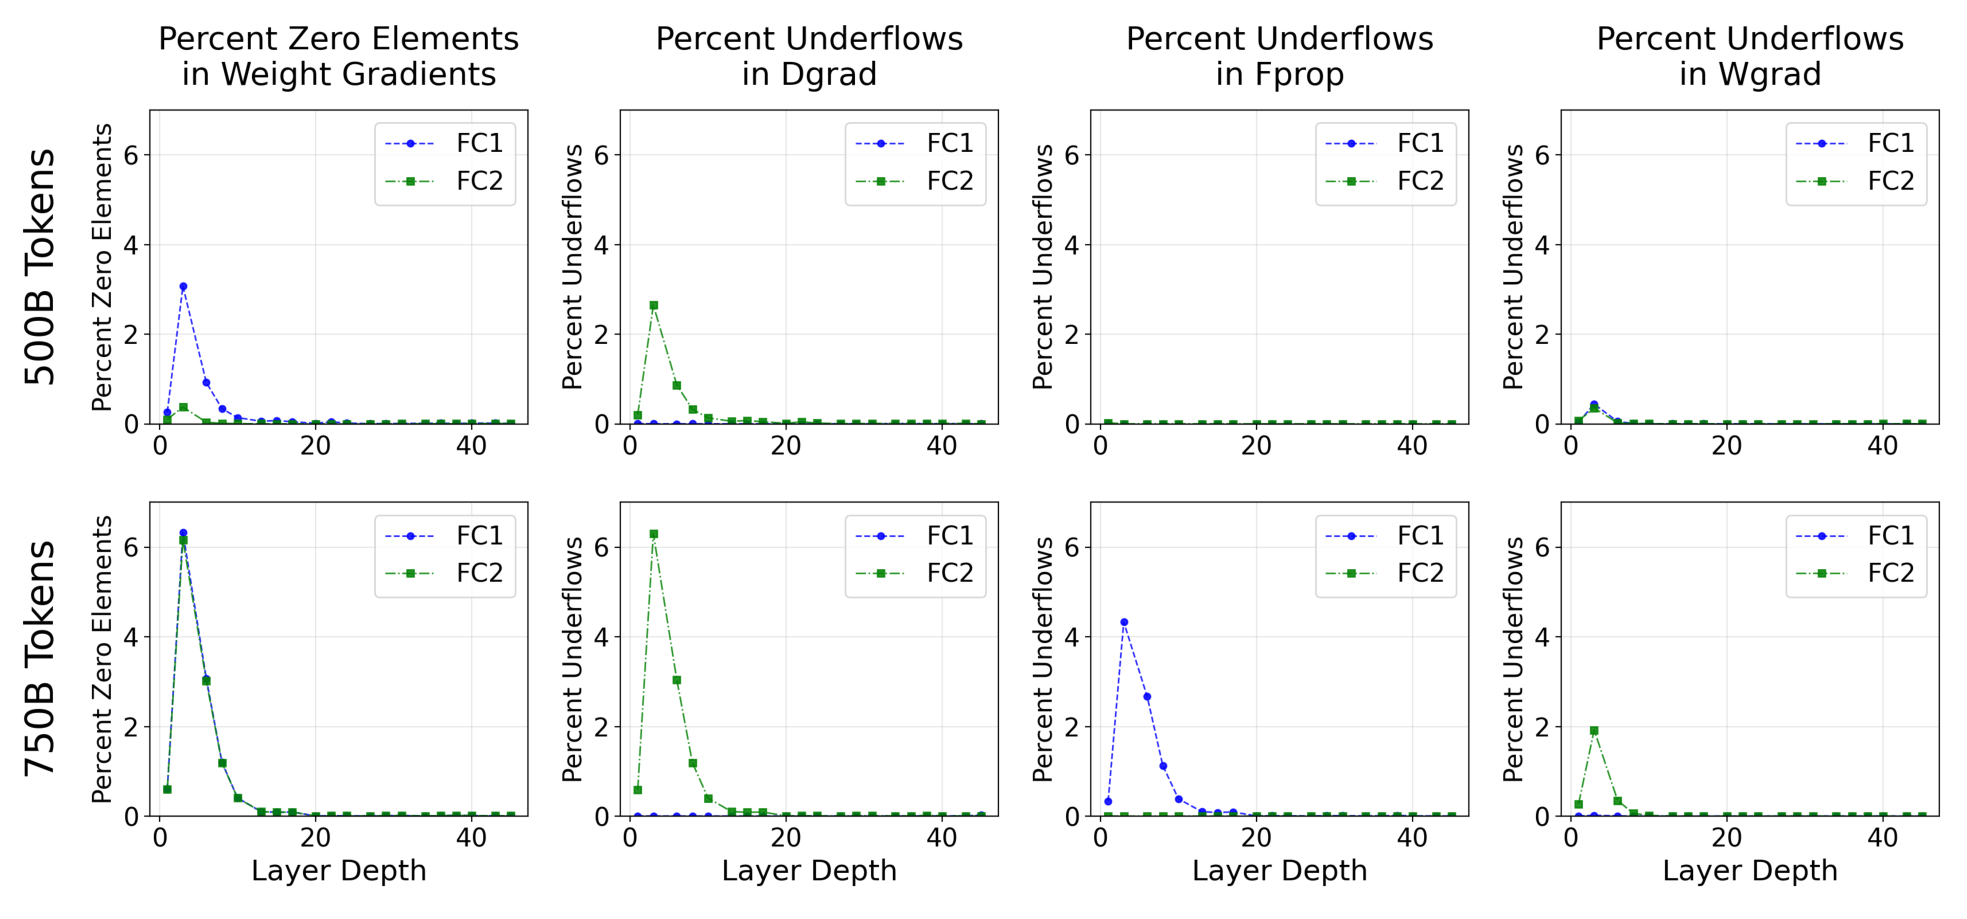
\includegraphics[width=1\textwidth]{figures/nvfp4_wgrad_zeros.pdf}
    \caption{Origin of Zero Element Weight Gradients in Nemotron 3 Nano, shown for routed expert layers increasing in layer depth. Averaged across all routed experts in a layer index. Top: Tensors sampled at 500B tokens. Percent of zero-valued weight gradients are higher for FC1 than FC2 and attributed almost entirely to underflows in dgrad of FC2. Bottom: Tensors sampled at 750B tokens. Percent of zero-valued weight gradients are equivalently high for FC1 and FC2. Zero-valued weight gradients in FC1 are attributed to underflows in dgrad of FC2. Zero element weight gradients in FC2 are attributed mainly to underflows in fprop of FC1, with a minor contribution of underflows in wgrad of FC2.}
    \label{fig:nvfp4_wgrad_zeros}
\end{figure}




Following our previous work in NVFP4 pretraining \citep{nvidia2025pretraininglargelanguagemodels}, we evaluated whether switching all tensors to higher precision prior to learning rate annealing would benefit Nemotron 3 Super. We promoted all tensors to MXFP8 at 19T tokens (1T tokens before annealing) and continued training through 20.6T tokens. While this improved the loss trajectory, it yielded no gains in downstream task accuracy (Fig \ref{fig:nvfp4_healing_super}). The final Nemotron 3 Super model is therefore pretrained with our NVFP4 recipe for the entire token horizon. 


\begin{figure}[h!]
    \centering
    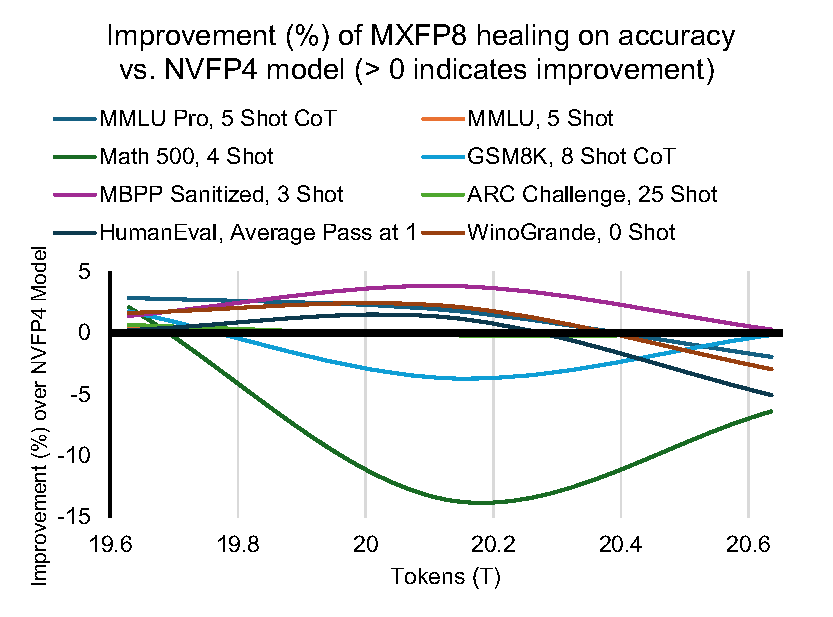
\includegraphics[width=0.65\textwidth]{figures/nvfp4_healing_super.pdf}
    \caption{Improvement in downstream task evaluation accuracy after switching the network precision to MXFP8. Values greater than zero indicate improvement in accuracy over the NVFP4 model. None of the downstream task evaluation metrics showed sustained improvement after training in MXFP8.}
    \label{fig:nvfp4_healing_super}
\end{figure}